\documentclass[a4paper, 10pt]{article}
\usepackage{../../CEDT-Homework-style}

\usepackage{amsmath}
\allowdisplaybreaks

\setlength{\headheight}{14.49998pt}

\begin{document}
\subject[2110203 - Computer Engineering Mathematics II]
\hwtitle{Signal 1 (for assignment)}{}{Week 1}{6733172621 Patthadon Phengpinij}{ChatGPT (for\,\LaTeX\,styling and grammar checking)}


% ================================================================================ %
\section{Representing Signals}
% ================================================================================ %



% ================================================================================ %
%                                    Problem 01                                    %
% ================================================================================ %
\begin{problem}
Sketch the following signals
\end{problem}

% === Problem 1.1. === %

\begin{tosubmit}
\begin{subproblems}
    \item \( x(t) = \sin \paren{\frac{\pi}{4} t + 20^\circ} \)
\end{subproblems}

\par\noindent\submitsolution
Using Python and Matplotlib to plot the signal \( x(t) = \sin \paren{\frac{\pi}{4} t + 20^\circ} \):
\begin{codingbox}
import matplotlib.pyplot as plt
import numpy as np

fig = plt.figure()

t = np.arange(-10, 10, 0.01)
x = np.sin(np.pi/4 * t + np.pi/9)

plt.title("Problem 1.1")
plt.plot(t, x, label=r"$x(t) = \sin(\frac{\pi}{4}t + 20^\circ)$")
plt.legend(loc="upper right")
plt.grid(True)
plt.show()
\end{codingbox}

The plot of the signal is shown below:
\begin{center}
    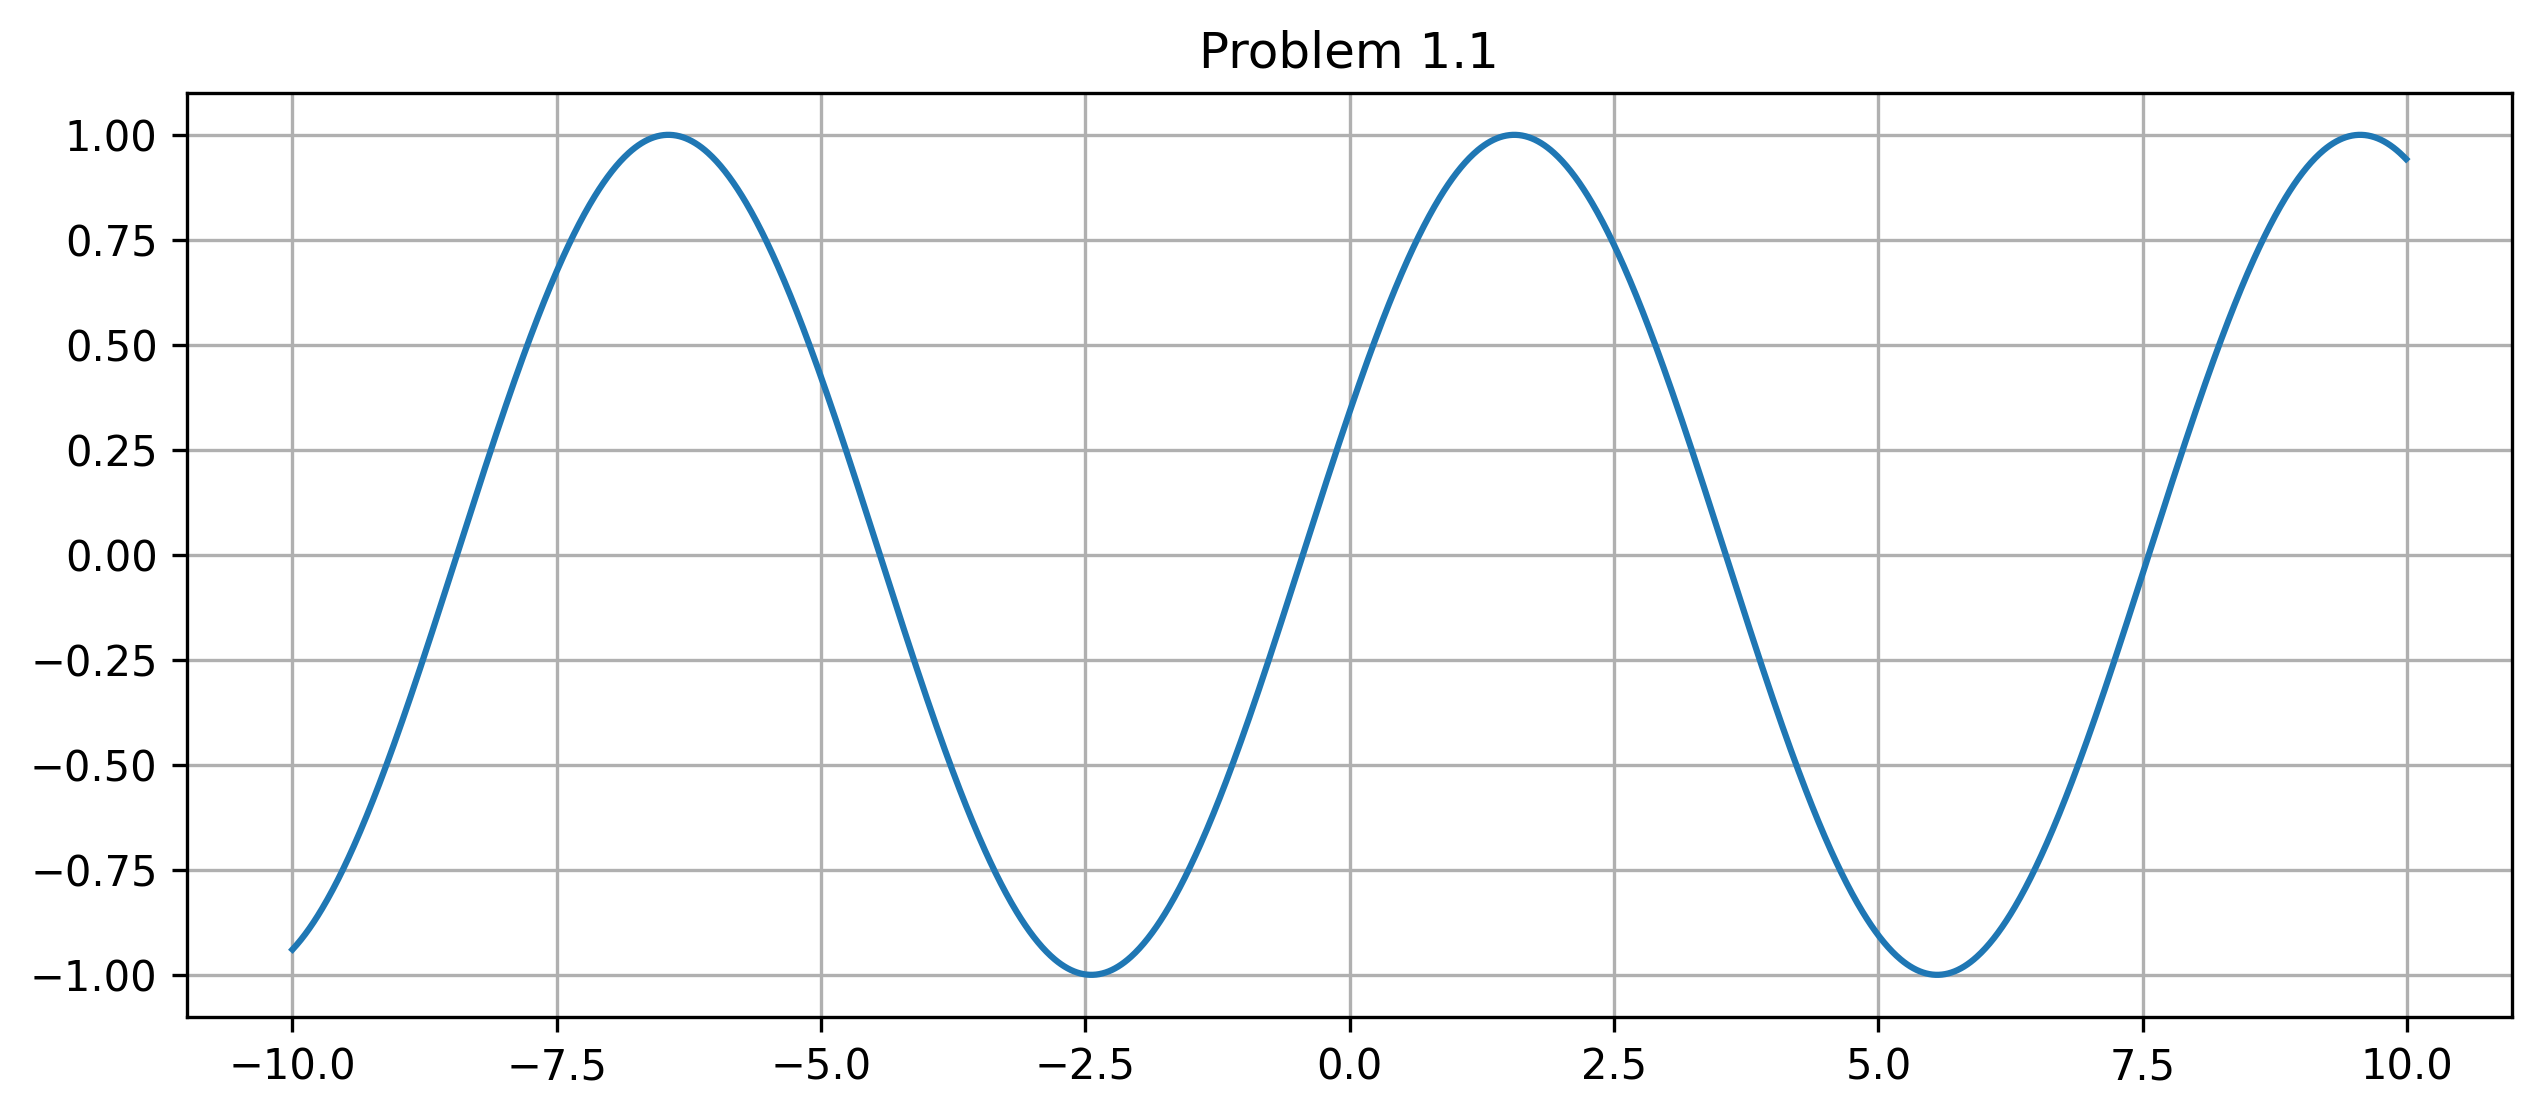
\includegraphics[width=0.8\textwidth]{images/problem_1_1.png}
\end{center}
\end{tosubmit}

% ==================== %

\newpage

% === Problem 1.3. === %
\begin{tosubmit}
\begin{subproblems}[start=3]
    \item \( x(t) = 2e^{-t}, 0 \leq t < 1 \text{ and } x(t + 1) = x(t), \forall t \)
\end{subproblems}

\par\noindent\submitsolution
Using Python and Matplotlib to plot the piecewise signal \( x(t) = 2e^{-t}, 0 \leq t < 1 \text{ and } x(t + 1) = x(t), \forall t \):
\begin{codingbox}
import matplotlib.pyplot as plt
import numpy as np

def x3(t):
    if t >= 1:
        return x3(t - 1)
    if t < 0:
        return x3(t + 1)
    return 2 * (np.e ** (-t))

fig = plt.figure(figsize=(10, 4))

t = np.arange(-10, 10, 0.01)
x3_vectorize = np.vectorize(x3)
x = x3_vectorize(t)

plt.title("Problem 1.3")
plt.plot(t, x, label=r"$x(t) = 2e^{-t}, 0 \leq t < 1 \text{ and } x(t + 1) = x(t), \forall t$")
plt.legend(loc="upper right")
plt.grid(True)
plt.show()
\end{codingbox}

The plot of the signal is shown below:
\begin{center}
    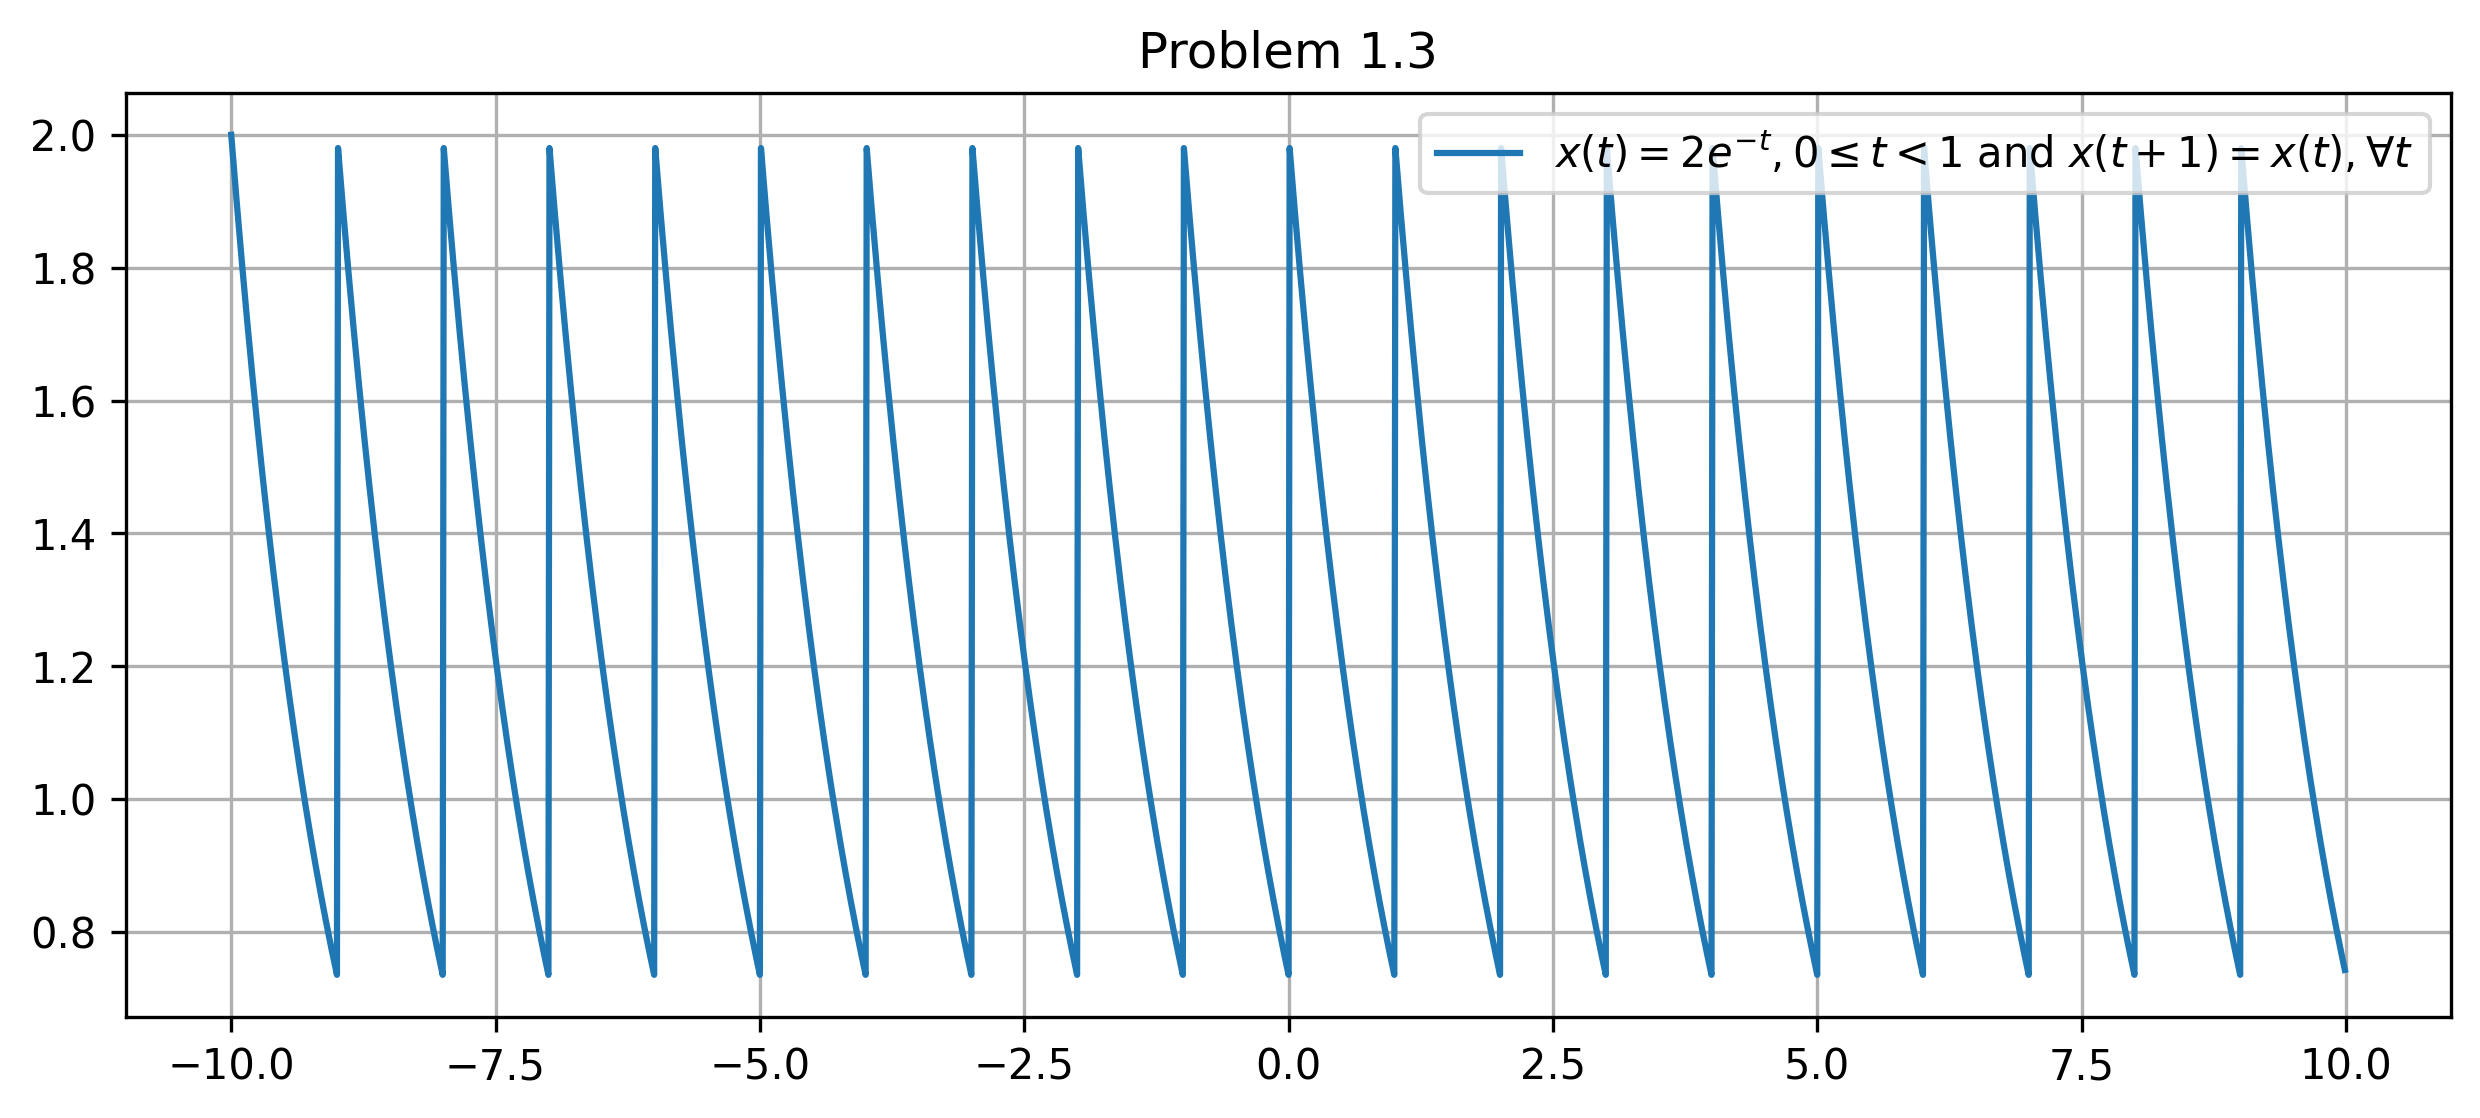
\includegraphics[width=0.8\textwidth]{images/problem_1_3.png}
\end{center}
\end{tosubmit}
% ==================== %

\newpage

% === Problem 1.5. === %
\begin{tosubmit}
\begin{subproblems}[start=5]
    \item \( x(t) = r(t) - r(t - 1) - u(t - 2) \)
\end{subproblems}

\par\noindent\submitsolution
Using Python and Matplotlib to plot the piecewise signal \( x(t) = r(t) - r(t - 1) - u(t - 2) \):
\begin{codingbox}
import matplotlib.pyplot as plt
import numpy as np

def unit_signal(t):
    return 1.0 if t >= 0 else 0.0

def ramp_signal(t):
    return t * unit_signal(t)

unit_signal_vectorize = np.vectorize(unit_signal)
ramp_signal_vectorize = np.vectorize(ramp_signal)

fig = plt.figure(figsize=(10, 4))

t = np.arange(-2, 4, 0.01)

r1 = ramp_signal_vectorize(t)
r2 = ramp_signal_vectorize(t - 1)
u1 = unit_signal_vectorize(t - 2)

x = r1 - r2 - u1

plt.title("Problem 1.5")
plt.plot(t, x, label=r"$r(t) - r(t-1) - u(t-2)$")
plt.legend(loc="upper right")
plt.grid(True)
plt.show()
\end{codingbox}

The plot of the signal is shown below:
\begin{center}
    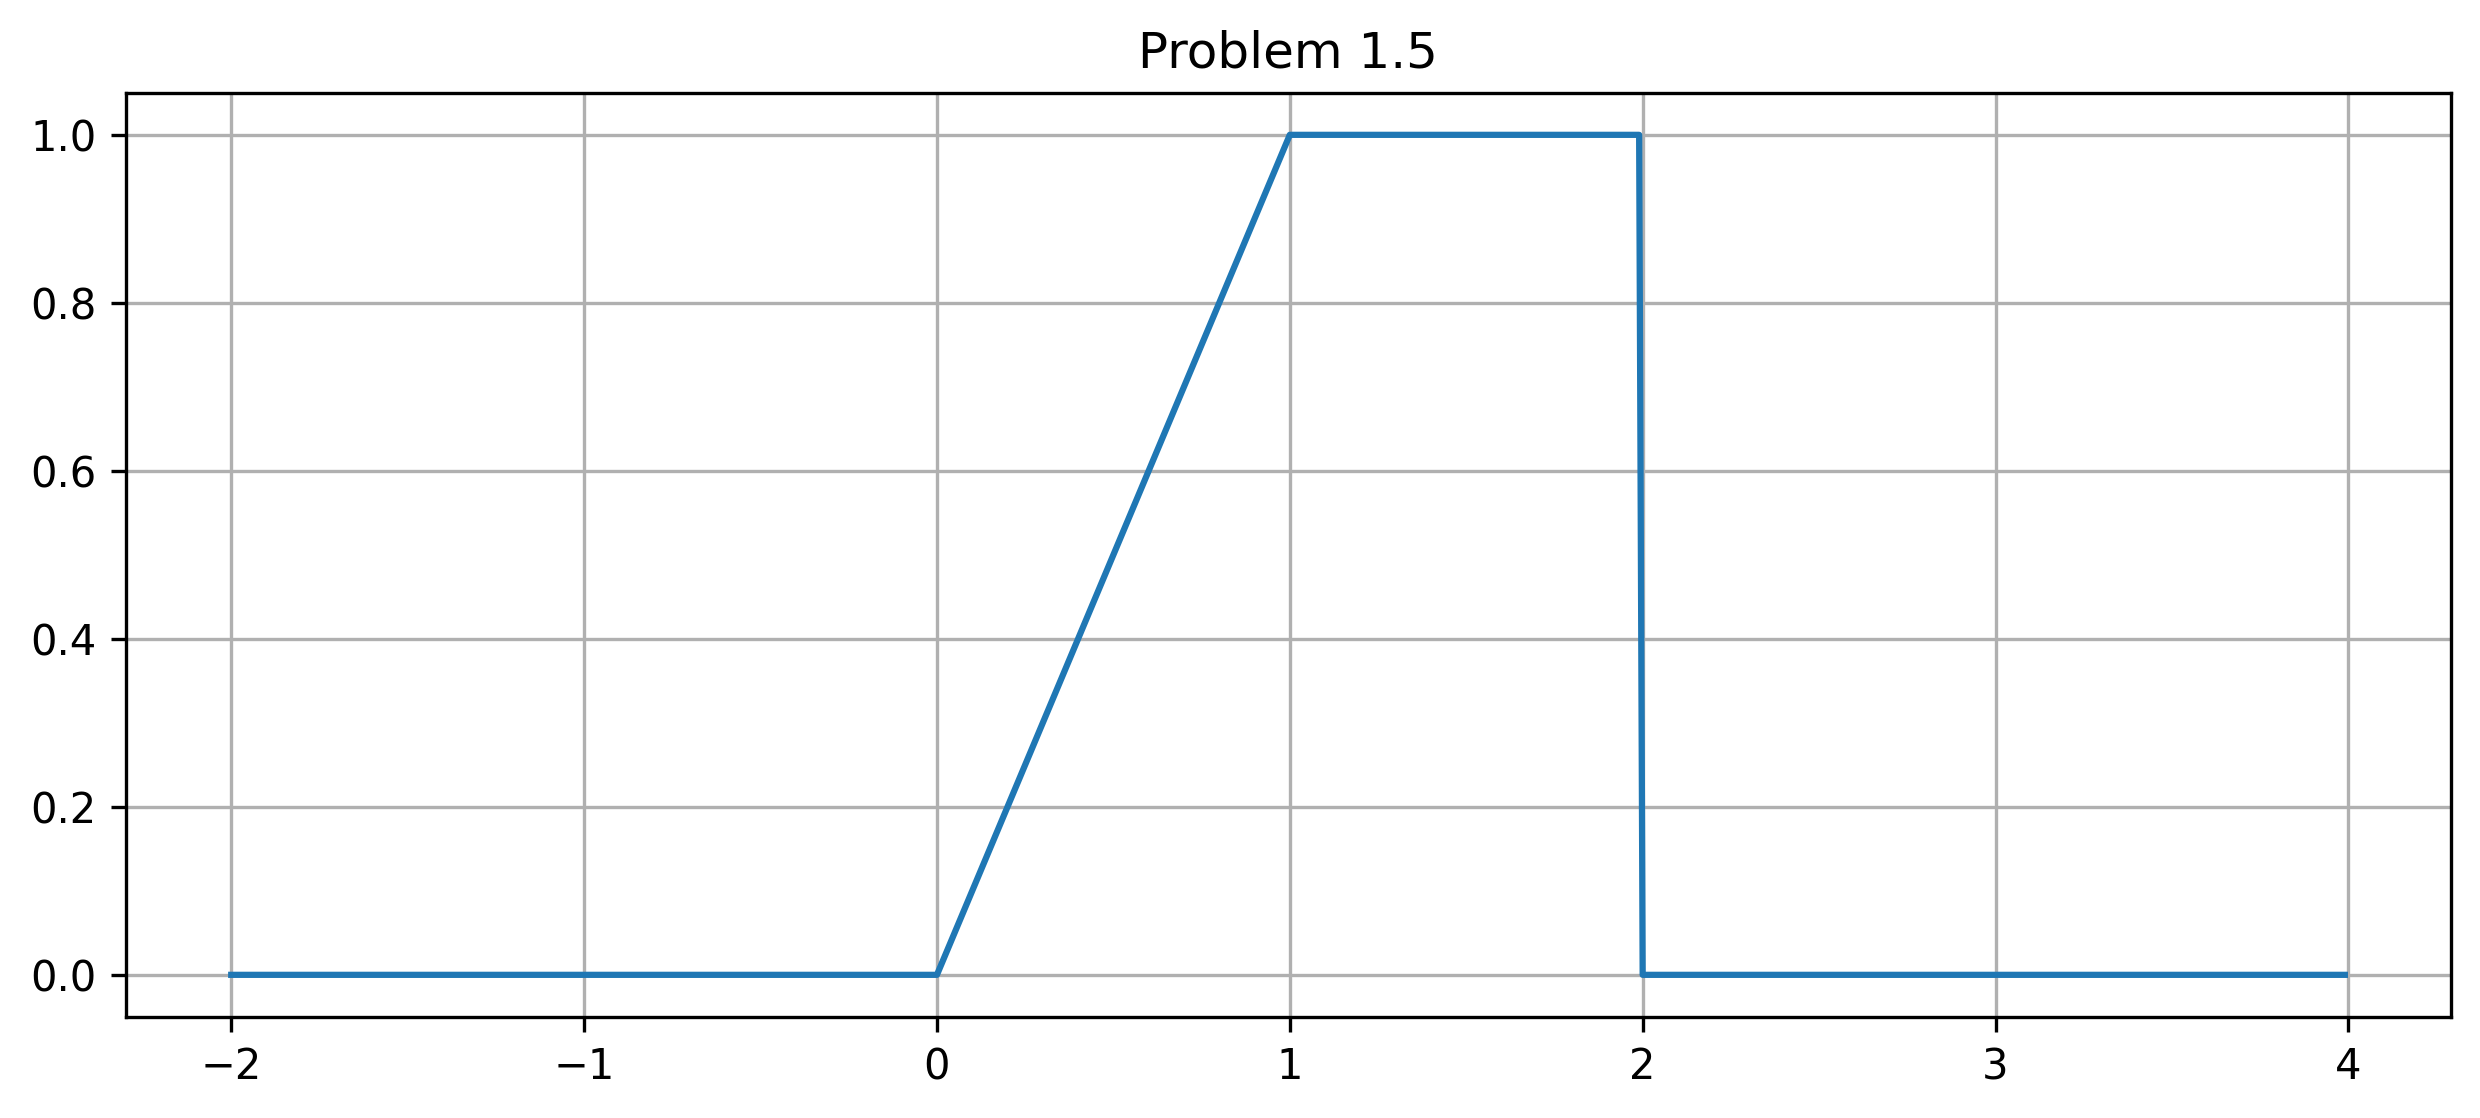
\includegraphics[width=0.8\textwidth]{images/problem_1_5.png}
\end{center}
\end{tosubmit}
% ==================== %

% ================================================================================ %

\newpage

% ================================================================================ %
%                                    Problem 04                                    %
% ================================================================================ %
\begin{problem}
For the discrete time signal \( x[n] \) shown in Figure below, sketch each of the following

\begin{codingbox}
import matplotlib.pyplot as plt
import numpy as np

fig = plt.figure(figsize=(6, 4))

t = np.arange(-2, 4)
x_t = np.array([-3, 1, 2, -2, 3, -1])

plt.stem(t, x_t)
plt.title(r"$x[n]$")
plt.show()
\end{codingbox}

With the resulting plot shown below:
\begin{center}
    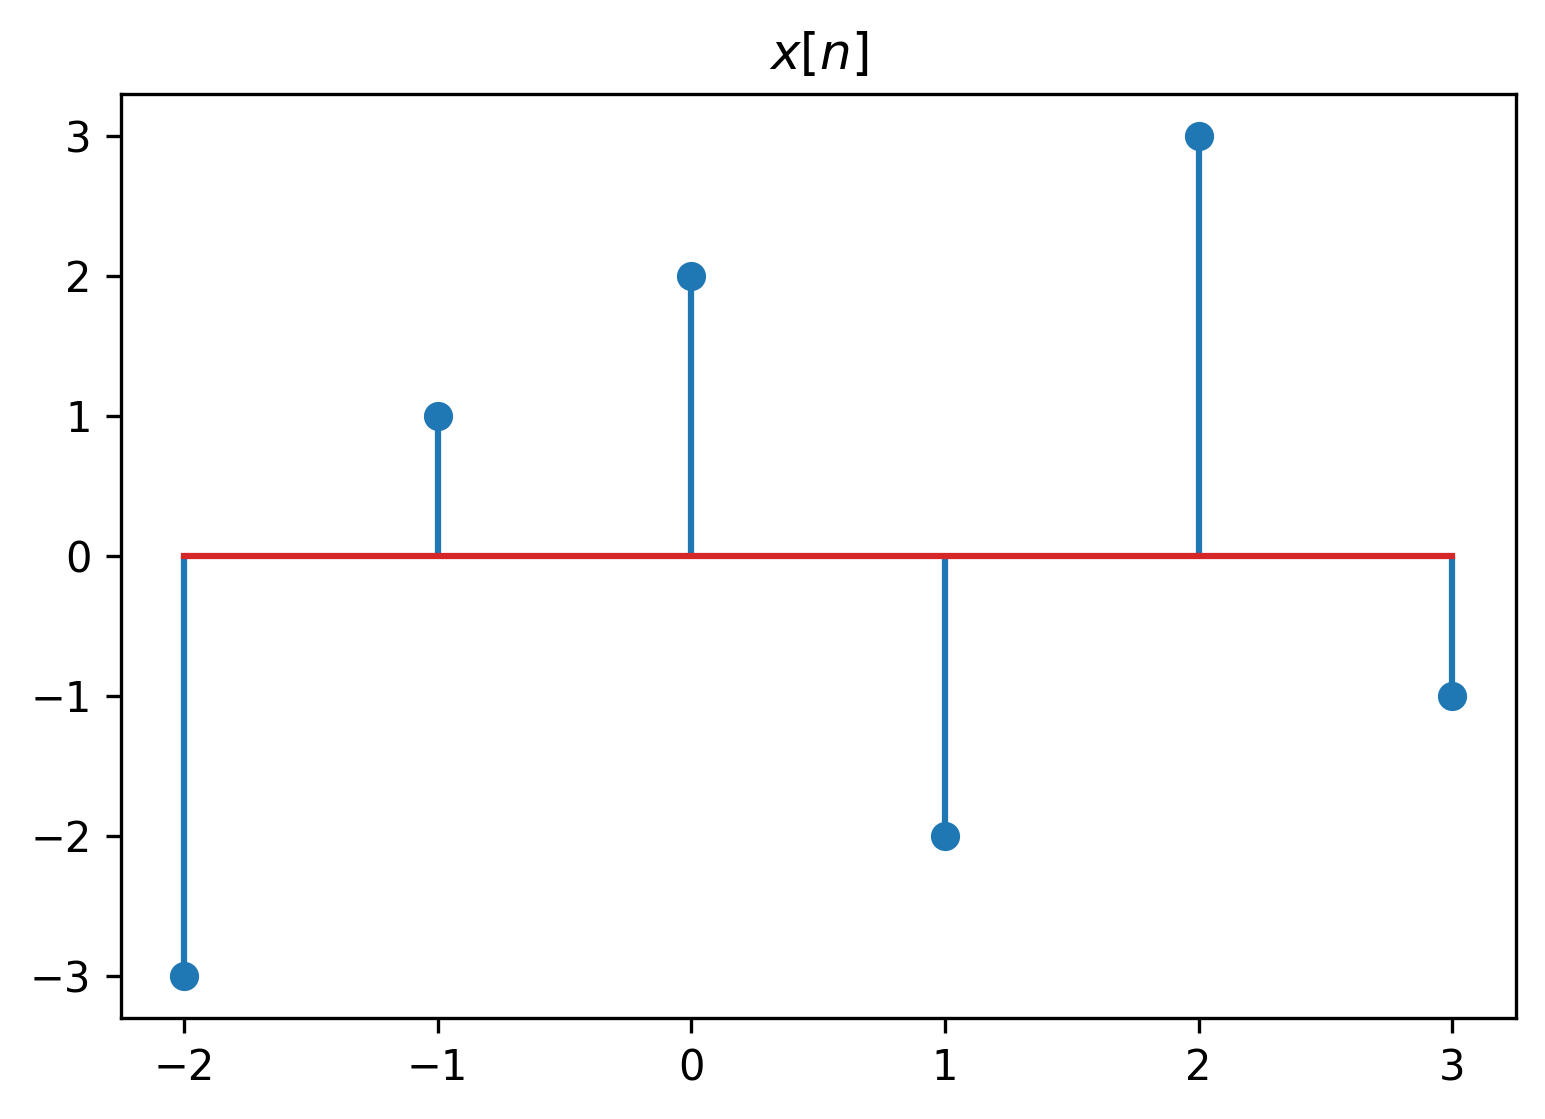
\includegraphics[width=0.5\textwidth]{images/problem_4_xn.png}
\end{center}
\end{problem}

\begin{solution}
By using Python, we can create a function to transform the signal based on the given transformation function:
\begin{codingbox}
def transform_signal(x, n, f):
    """Return x[f(n)] for any discrete-time signal x[n]."""
    f_n = f(n)
    f_n_int = f_n[np.floor(f_n) == f_n]
    
    x_new = np.zeros(f_n_int.shape[0], dtype=float)
    
    idx = 0
    for i, val in enumerate(f_n):
        if int(val) == val:
            x_new[idx] = x[i]
            idx += 1
    
    return x_new, f_n_int
\end{codingbox}
\end{solution}

\newpage

% === Problem 4.1. === %
\begin{tosubmit}
\begin{subproblems}
    \item \( x[2-n] \)
\end{subproblems}

\par\noindent\submitsolution
Using Python and Matplotlib to plot the signal \( x[2-n] \):
\begin{codingbox}
import matplotlib.pyplot as plt
import numpy as np

fig = plt.figure(figsize=(6, 4))

t = np.arange(-2, 4)
x_t = np.array([-3, 1, 2, -2, 3, -1])

x_t, t = transform_signal(x_t, t, lambda x: 2 - x)

plt.stem(t, x_t)
plt.title(r"$x[2 - n]$")
plt.show()
\end{codingbox}

With the resulting plot shown below:
\begin{center}
    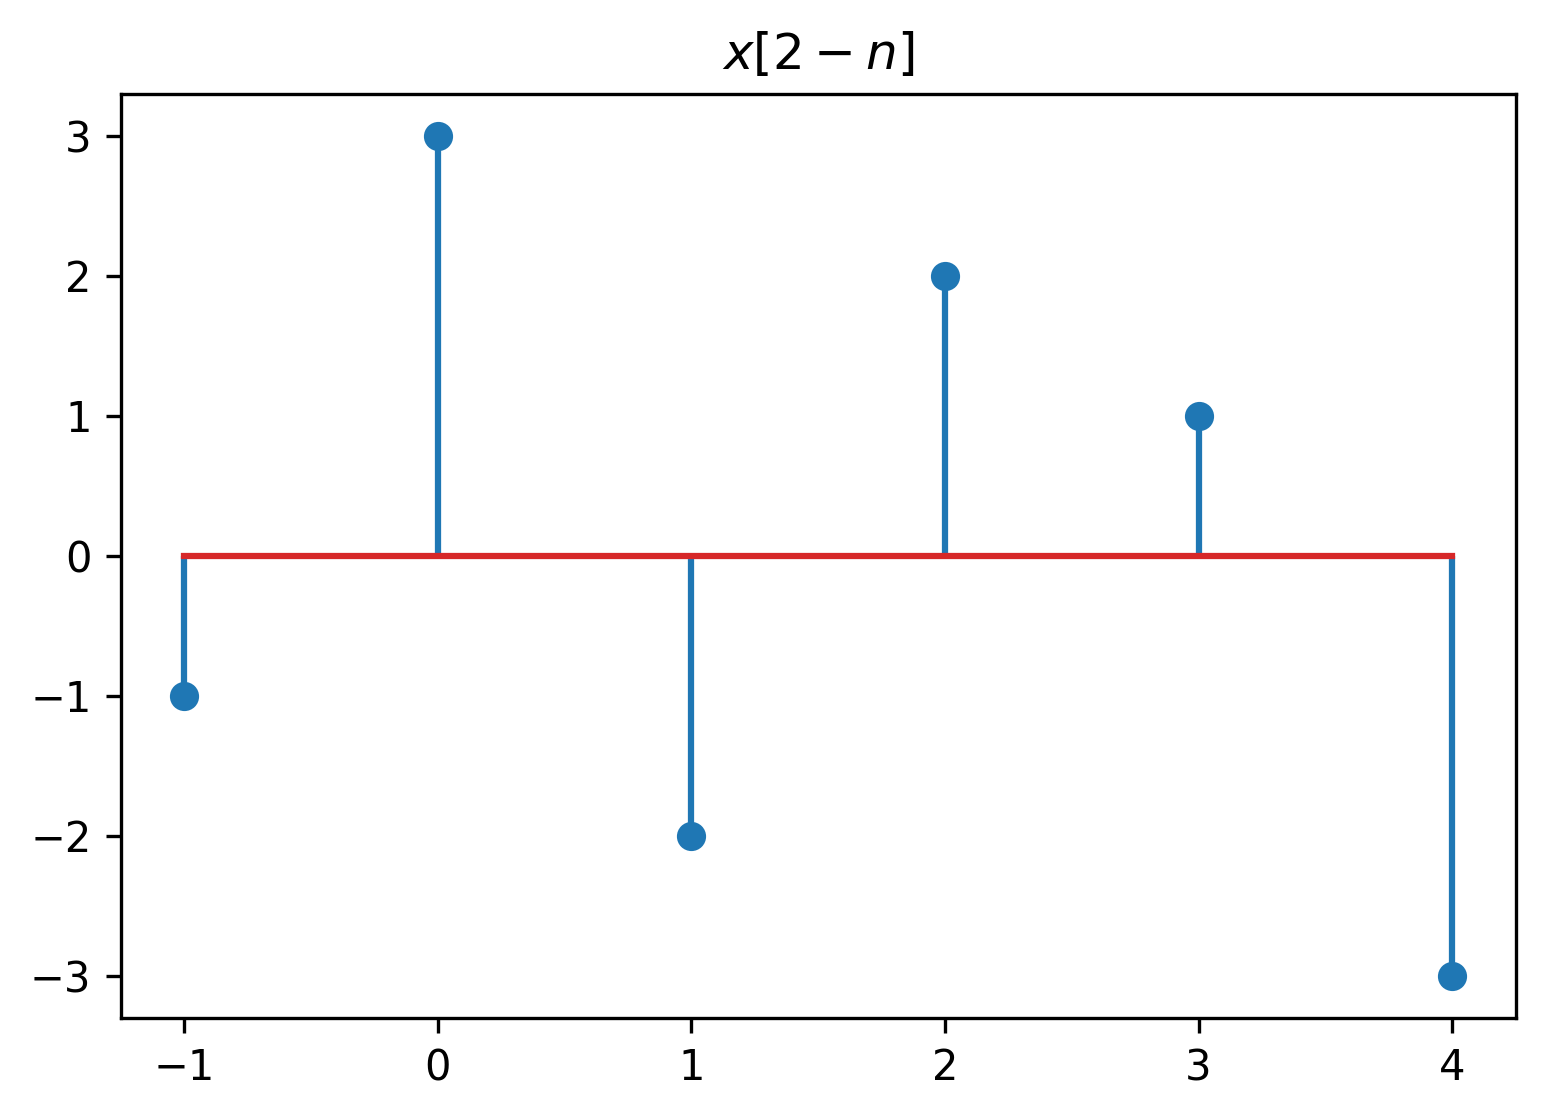
\includegraphics[width=0.5\textwidth]{images/problem_4_1.png}
\end{center}
\end{tosubmit}
% ==================== %

% === Problem 4.3. === %
\begin{tosubmit}
\begin{subproblems}[start=3]
    \item \( x\sqbracket{\frac{2}{3}n+1} \)
\end{subproblems}

\par\noindent\submitsolution
Using Python and Matplotlib to plot the signal \( x[\frac{2}{3}n+1] \):
\begin{codingbox}
import matplotlib.pyplot as plt
import numpy as np

fig = plt.figure(figsize=(6, 4))

t = np.arange(-2, 4)
x_t = np.array([-3, 1, 2, -2, 3, -1])

x_t, t = transform_signal(x_t, t, lambda x: (x - 1) * 3 / 2)

plt.stem(t, x_t)
plt.title(r"$x[\frac{2}{3}n + 1]$")
plt.show()
\end{codingbox}

\newpage

With the resulting plot shown below:
\begin{center}
    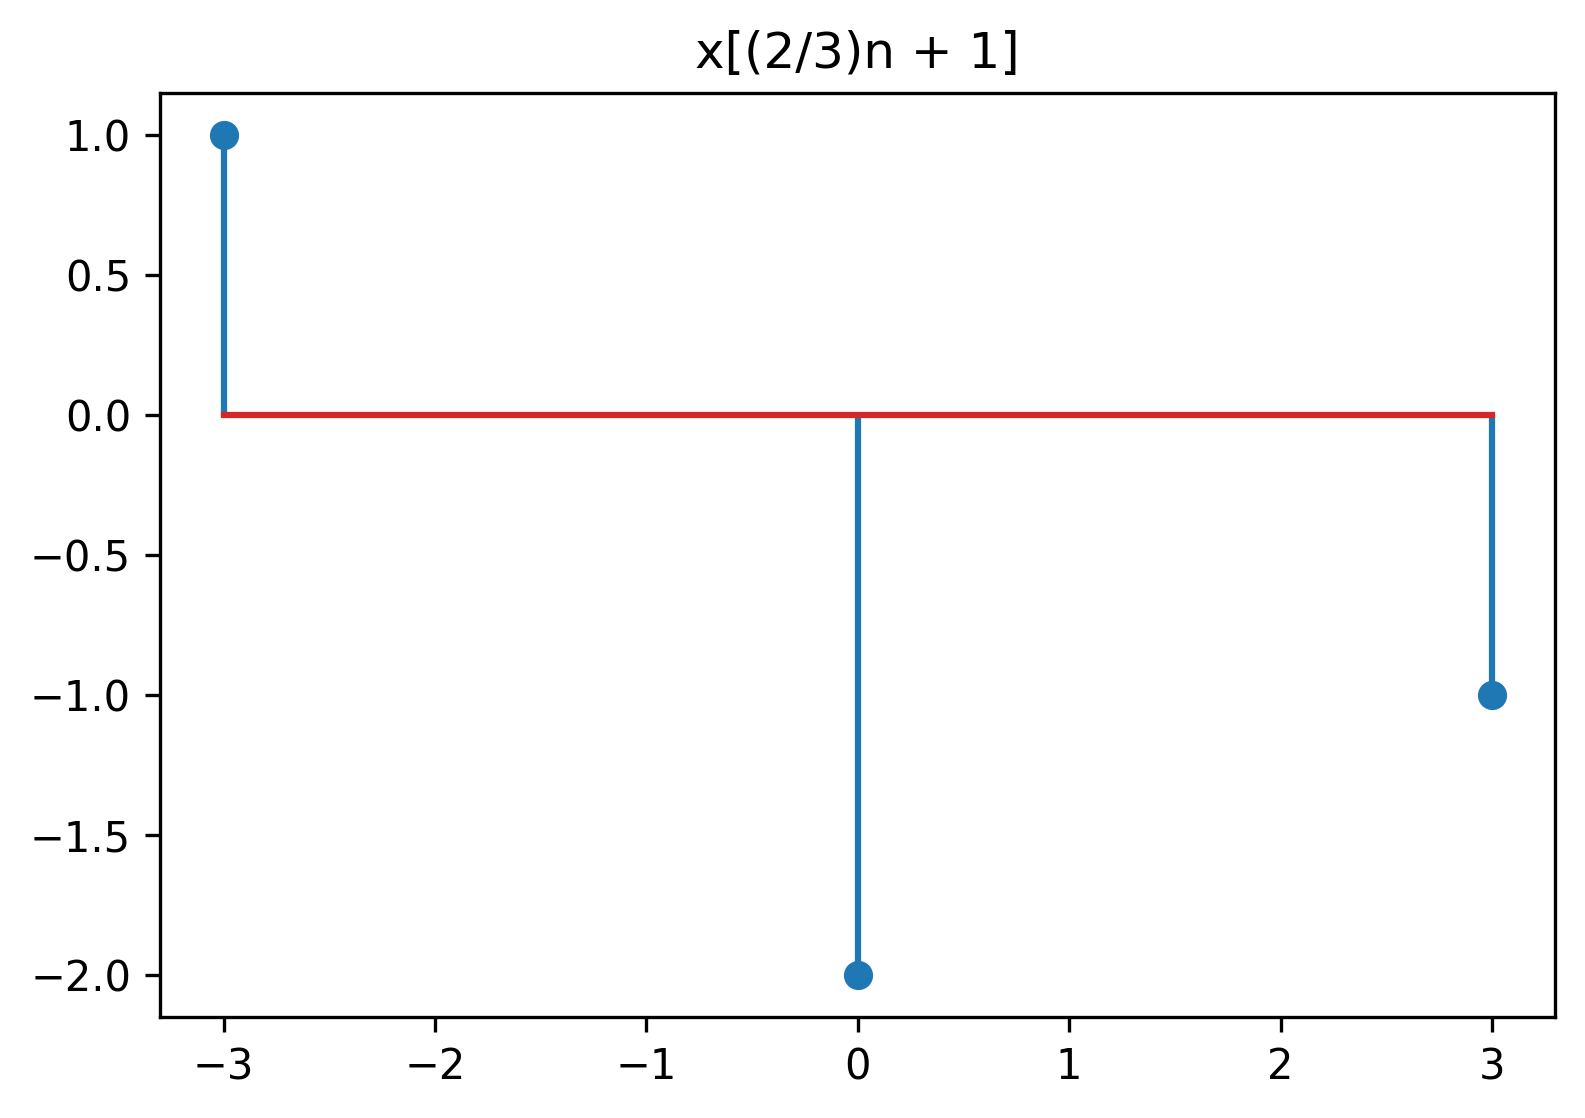
\includegraphics[width=0.5\textwidth]{images/problem_4_3.png}
\end{center}
\end{tosubmit}
% ==================== %


% === Problem 4.5. === %
\begin{tosubmit}
\begin{subproblems}[start=5]
    \item \( x[n^3] \)
\end{subproblems}

\par\noindent\submitsolution
Using Python and Matplotlib to plot the signal \( x[n^3] \):
\begin{codingbox}
import matplotlib.pyplot as plt
import numpy as np

fig = plt.figure(figsize=(6, 4))

t = np.arange(-2, 4)
x_t = np.array([-3, 1, 2, -2, 3, -1])

x_t, t = transform_signal(x_t, t, lambda x: np.cbrt(x))

plt.stem(t, x_t)
plt.title(r"$x[n^3]$")
plt.show()
\end{codingbox}

With the resulting plot shown below:
\begin{center}
    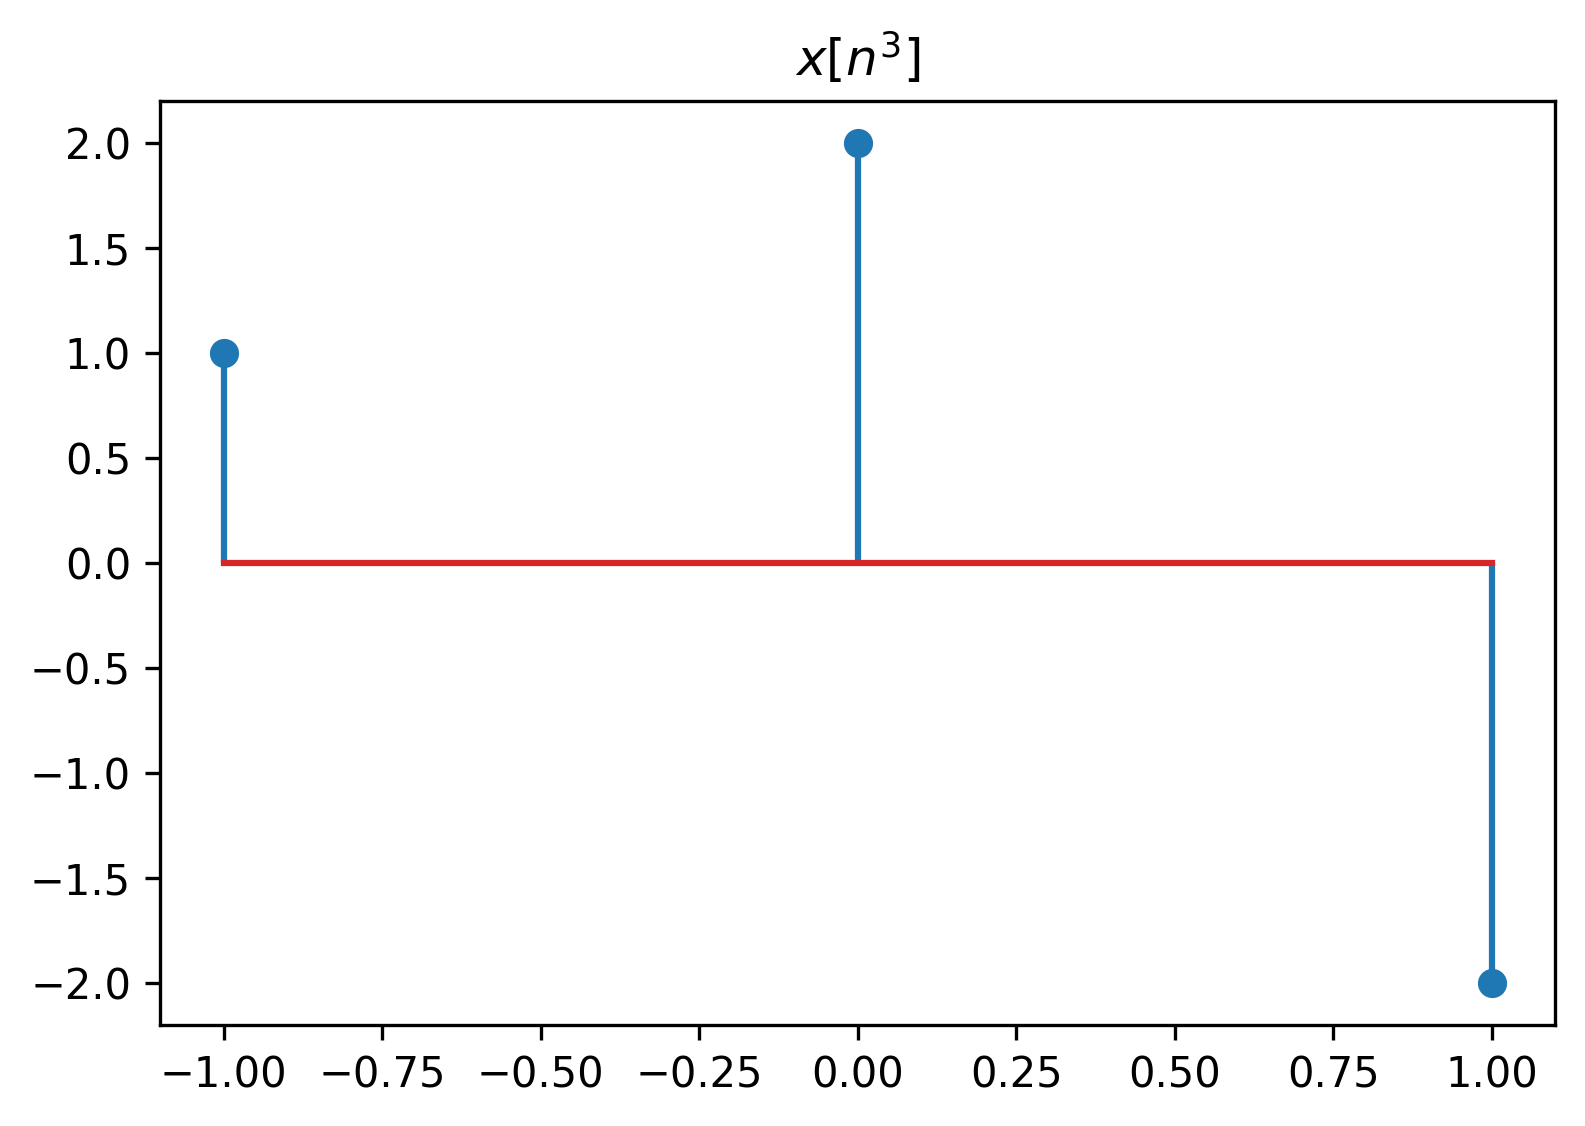
\includegraphics[width=0.5\textwidth]{images/problem_4_5.png}
\end{center}
\end{tosubmit}
% ==================== %

\newpage

% ================================================================================ %
%                                    Problem 09                                    %
% ================================================================================ %
\begin{problem}[9]
Evaluate the following integrals
\end{problem}

% === Problem 9.1. === %
\begin{tosubmit}
\begin{subproblems}
    \item \( \int_{-\infty}^{\infty} \paren{\frac{2}{3}t-\frac{3}{2}} \delta(t-1) \,dt \)
\end{subproblems}

\par\noindent\submitsolution
Using the sifting property of the delta function, we have:
\begin{align*}
    \int_{-\infty}^{\infty} \paren{\frac{2}{3}t-\frac{3}{2}} \delta(t-1) \,dt &= \paren{\frac{2}{3}(1)-\frac{3}{2}} \\
    &= \frac{2}{3} - \frac{3}{2} \\
    \int_{-\infty}^{\infty} \paren{\frac{2}{3}t-\frac{3}{2}} \delta(t-1) \,dt &= \boxed{-\frac{5}{6}}
\end{align*}
\end{tosubmit}
% ==================== %


% === Problem 9.3. === %
\begin{tosubmit}
\begin{subproblems}[start=3]
    \item \( \int_{-3}^{-2} \sqbracket{ e^{(-t+1)} + \sin \paren{ \frac{2\pi t}{3} } } \delta \paren{t- \frac{3}{2} } \,dt \)
\end{subproblems}

\par\noindent\submitsolution
Because the argument of the delta function \( t - \frac{3}{2} \) has its root at \( t = \frac{3}{2} \), which is outside the integration limits of -3 to -2, the integral evaluates to zero:
\begin{align*}
    \int_{-3}^{-2} \sqbracket{ e^{(-t+1)} + \sin \paren{ \frac{2\pi t}{3} } } \delta \paren{t- \frac{3}{2} } \,dt &= \boxed{0}
\end{align*}
\end{tosubmit}
% ==================== %
% ================================================================================ %


\end{document}